\chapter{Algoritmo di inferenza}

\section{Sommario}

\dfn{Fasi dell'algoritmo}{
\begin{enumerate}
    \item Si costrusce l'albero sintattico della $\lambda$-espressione;
    \item Si annota l'albero e si generano i vincoli:
    \begin{itemize}
        \item variabile di tipo: tipo sconosciuto;
        \item espressione di tipo: tipo (parzialmente) sconosciuto;
        \item vincolo: relazione di uguaglianza tra tipi espressa nelle regole di tipo.
    \end{itemize}
    \item Si risolvono i vincoli: 
    \begin{itemize}
        \item Si deve determinare se il sistema ammette almeno una soluzione;
        \item Si deve calcolare la soluzione più generale da cui derivare tutte le altre.
    \end{itemize}
\end{enumerate}
}

\subsection{Costruzione dell'albero sintattico}

\begin{itemize}
    \item Si rappresenta la $\lambda$-espressione come un albero;
    \item I nodi interni e le foglie sono opportunamente etichettati;
    \item Indichieamo con T[M] l'albero corrispondente alla $\lambda$-espressione.
\end{itemize}

\dfn{Albero sintattico}{
\begin{itemize}
    \item $T[x] = x$ (foglia);
    \item $T[c] = c$ (foglia);
    \item $T[\lambda x.M] =$
    \begin{forest}
        [$\lambda x$ [$T{[M]}$]]
    \end{forest}
    \item $T [M\:\:N] =$
    \begin{forest}
        [@ [$T{[M]}$][$T{[N]}$]]
    \end{forest}
    \item $T[\text{\textcolor{red}{ if }} M\:\:N_1\:\:N_2] =$
    \begin{forest}
        [\textcolor{red}{if}[$T{[M]}$][$T{[N_1]}$][$T{[N_2]}$]]
    \end{forest}
\end{itemize}
}

\ex{}{
\begin{multicols}{2}

    \begin{itemize}
        \item $(\lambda x. y)$ \textcolor{red}{True}
    \end{itemize}
    \begin{center}
        
    \begin{forest}
        [@ [$\lambda x$ [$x$]][\textcolor{red}{True}]]
    \end{forest}    \end{center}
\pagebreak
    \begin{itemize}
        \item \textcolor{red}{if True } $(\lambda x.x)\:\:(\lambda x.\lambda y.y)$
    \end{itemize}
    \begin{center}
            \begin{forest}
        [\textcolor{red}{if}[\textcolor{red}{True}][$\lambda x$[$x$]][$\lambda x$ [$\lambda y$ [$y$]]]]
    \end{forest}
    \end{center}
\end{multicols}

}

\subsection{Annotazione dell'albero e generazione dei vincoli}

\begin{itemize}
    \item Ogni nodo dell'albero viene annotato con un'espressione di tipo;
    \item Si procede in modo bottom-up, dalle foglie verso la radice.
\end{itemize}

\dfn{Sintassi delle espressioni di tipo}{Sia $TVar =\{\alpha,\:\beta,\:\gamma,\:...\}$ un insieme infinito di variabili di tipo e $\alpha$ un tipo sconosciuto\footnote{Ancora da determinare}, le espressioni di tipo $\tau,\:\sigma ::=$

$$\alpha \text{ (variabile di tipo)}$$
$$\text{\textcolor{green}{Bool} (booleani)}$$
$$\tau \rightarrow \sigma \text{ (funzioni)}$$
}

\nt{Un vincolo è una coppia di espressioni di tipo scritta come $\tau = \sigma$}
\begin{center}
    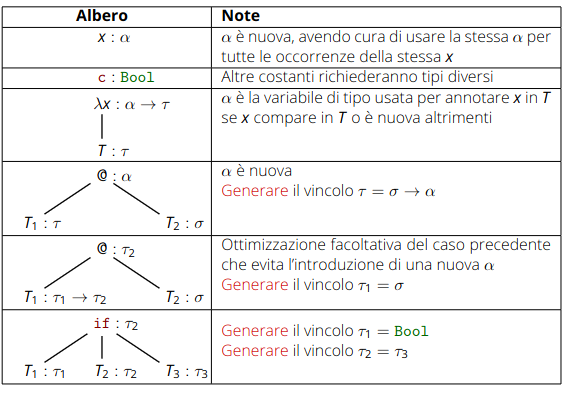
\includegraphics[scale = 0.7]{images/algoritmo di inferenza/Annotazione e vincoli.png}    
\end{center}

\ex{}{
\begin{multicols}{2}
[$\lambda x.x \:\:\text{\textcolor{red}{ True}}$]
    Albero annotato
    \begin{center}
    \begin{forest}
        [@ : \textcolor{red}{$\alpha$} [$\lambda x$ : \textcolor{red}{$\alpha \rightarrow \alpha$} [$x$ : \textcolor{red}{$\alpha$}]][True : \textcolor{green}{Bool}]]        
    \end{forest}
    \end{center}
    \pagebreak
    Vincoli generati

    $\alpha = \text{\textcolor{green}{Bool}}$
\end{multicols}
}

\ex{}{
\begin{multicols}{2}
[$\lambda f.\lambda x.f\:\:(f\:\:x)$]
    Albero annotato
    \begin{center}
    \begin{forest}
        [$\lambda f$ : \textcolor{red}{$\alpha \rightarrow \beta \rightarrow \delta$}[$\lambda x$ : \textcolor{red}{$\beta \rightarrow \delta$} [@ : \textcolor{red}{$\delta$}[$f$ : \textcolor{red}{$\alpha$}] [@ : \textcolor{red}{$\gamma$} [$f$ : \textcolor{red}{$\alpha$}] [$x$ : \textcolor{red}{$\beta$}]]]]]
    \end{forest}
    \end{center}
    \pagebreak
    Vincoli generati

    $\alpha = \beta \rightarrow \gamma$

    $\alpha = \gamma \rightarrow \delta$
\end{multicols}
}

\nt{Nell'ultimo esempio entrambe le $f$ hanno la stessa annotazione}

\subsection{Sistemi di equazioni e soluzioni}

\dfn{Sostituzione}{Una sostituzione $\theta$ è una funzione da variabili di tipo a espressioni di tipo. Scriviamo $\theta(\tau)$ per l'espressione ottenuta da $\tau$ sostituendo ogni $\alpha$ con $\theta (\alpha)$}

\dfn{Soluzione}{Dato un sistema di vincoli $\{\tau_i = \sigma_i\}_{1 \leq i \leq n}$ e una sostituzione $\theta$ diciamo che $\theta$ è soluzione (o unificatore) del sistema se $\theta(\tau_i) = \theta(\sigma_i)$ per ogni $1 \leq i \leq n$. Diciamo inoltre che $\theta$ è l’unificatore più generale del sistema
se ogni soluzione del sistema è ottenibile componendo $\theta$ con un’altra sostituzione}

\begin{center}
    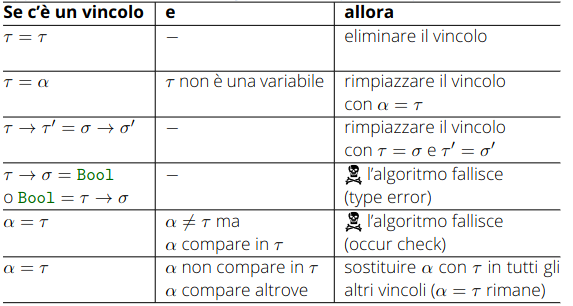
\includegraphics[scale = 0.7]{images/algoritmo di inferenza/Algoritmo di risoluzione.png}    
\end{center}

\nt{L'ordine in cui si applicano le trasformazioni non è importante. Se non si può applicare nessuna trasformazione l'algoritmo ha avuto successo}

\mprop{}{
\begin{itemize}
    \item In un numero finito di passi l'algoritmo ha successo o fallisce;
    \item Se l'algoritmo fallisce allora il sistema è insoddisfacibile;
    \item Se l'algoritmo ha successo:
    \begin{itemize}
        \item il sistema ha forma $\{\alpha_i = p_i\}_{1 \leq i \leq m}$ in cui ciascuna $\alpha_i$ compare una sola volta nel sistema;
        \item la sostituzione $\theta = \{\alpha_i \rightarrow p_i\}_{1 \leq i \leq m}$ è l'unificatore più generale del sistema iniziale, in particolare $\sigma(\tau_i) = \theta(\sigma_i))$ per ogni $\ \leq i \leq m$.
    \end{itemize}
\end{itemize}
}
\pagebreak
\ex{}{
\begin{center}
    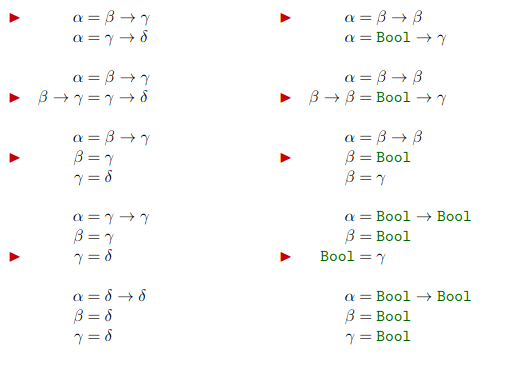
\includegraphics[scale = 0.7]{images/algoritmo di inferenza/Esempio.png}    
\end{center}
}


\ex{Esercizio}{
$(\lambda x.\lambda y. x\:\:y\:\:y) (\lambda a.a) b)$
\begin{multicols}{2}
\begin{center}

    \begin{forest}
    [@ : \textcolor{red}{n} [@ : \textcolor{red}{$\beta \rightarrow$ n}[$\lambda x$ : \textcolor{red}{$\alpha \rightarrow \beta \rightarrow $n }[$\lambda y$ : \textcolor{red}{$\beta \rightarrow$ n}[@ : \textcolor{red}{n}[@ : \textcolor{red}{$\epsilon$} [x : \textcolor{red}{$\alpha$}][y : \textcolor{red}{$\beta$}]][y : \textcolor{red}{$\beta$}]]]][$\lambda$ a : \textcolor{red}{$\gamma \rightarrow \gamma$}[a : \textcolor{red}{$\gamma$}]]] [b : \textcolor{red}{$\sigma$}]]
    \end{forest}
    
\end{center}
\pagebreak
$\alpha = \beta \rightarrow \epsilon$

$\epsilon = \beta \rightarrow$ n

$\alpha = \gamma \rightarrow \gamma$

$\beta = \sigma$
\end{multicols}
\pagebreak
Risoluzione:
\begin{multicols}{2}
$\begin{cases}
    \alpha = \beta \rightarrow \epsilon\\

    \epsilon = \beta \rightarrow \text{n}\\

    \alpha = \gamma \rightarrow \gamma\\

    \beta = \sigma
\end{cases}$

$\begin{cases}
    \alpha = \beta \rightarrow \epsilon\\

    \epsilon = \beta \rightarrow \text{n}\\

    \beta \rightarrow \epsilon = \gamma \rightarrow \gamma\\

    \beta = \sigma
\end{cases}$

$\begin{cases}
    \alpha = \beta \rightarrow \epsilon\\

    \epsilon = \beta \rightarrow \text{n}\\

    \beta = \gamma\\

    \epsilon = \gamma \\

    \beta = \sigma
\end{cases}$

$\begin{cases}
    \alpha = \gamma \rightarrow \epsilon\\

    \epsilon = \gamma \rightarrow \text{n}\\

    \beta = \gamma\\

    \epsilon = \gamma \\

    \gamma = \sigma
\end{cases}$

$\begin{cases}
    \alpha = \gamma \rightarrow \gamma \rightarrow \text{n}\\

    \epsilon = \gamma \rightarrow \text{n}\\

    \beta = \gamma\\

    \gamma \rightarrow \text{n} = \gamma \\

    \gamma = \sigma
\end{cases}$

$\begin{cases}
    \alpha = \gamma \rightarrow \gamma \rightarrow \text{n}\\

    \epsilon = \gamma \rightarrow \text{n}\\

    \beta = \gamma\\

     \gamma = \gamma \rightarrow \text{n}\\

    \gamma = \sigma
\end{cases}$

\textcolor{red}{\textbf{! OCCUR CHECK FAIL !}}

\end{multicols}

}

\section{Estensioni dell'algoritmo}

\dfn{Numeri interi}{Le costanti includono i numeri interi
$$c \in \{\text{False}, \text{True}, \:\:0, \:\:1,...\}$$

Le espressioni di tipo sono arricchite con il tipo \textcolor{green}{Int}
}

\nt{Se c'è un vincolo $\tau \rightarrow \sigma = \text{\textcolor{green}{Int}}$ o \textcolor{green}{Int} = \textcolor{green}{Bool} o \textcolor{green}{Bool} = \textcolor{green}{Int} l'algoritmo fallisce (\textcolor{red}{TYPE ERROR})}

\dfn{Liste}{Le costanti includono i costruttori canonici
$$c \in \{..., \:\:[\:],\:\:(:)\}$$

Ogni occorrenza di un costruttore fa uso di nuove variabili di tipo
}

\nt{
\begin{itemize}
    \item Se c'è un vincolo $[\tau] = [\sigma]$ rimpiazzarlo con $\tau = \sigma$;
    \item Se c'è un vincolo $[\tau] = \text{\textcolor{green}{Bool}}$ o $\text{\textcolor{green}{Bool}} = [\tau]$ o $[\tau] = \sigma_1 \rightarrow \sigma_2$ o ... l'algoritmo fallisce (\textcolor{red}{TYPE ERROR})
\end{itemize}
}

\dfn{Funzioni di libreria}{Le costanti includono le funzioni di libreria
$$c \in \{...,\:\:\text{id},\:\:\text{head},\:\:\text{tail},...\}$$

Ogni occorrenza di una funzione di libreria fa uso di nuove variabili di tipo
}

\dfn{Definizioni ricorsive}{
$$f = M$$
dove $f$ può comparire in $M$.
Il nome $f$ è trattato come ogni altra variabile. Alla fine dell'annotazione si genera il vincolo $\alpha = \tau$ dove $\alpha$ è la variabile di tipo associata a $f$ e $\tau$ è l'annotazione di $M$
}






